\documentclass{article}
\usepackage[margin=0.5in]{geometry}
\usepackage{amsfonts}
\usepackage{amsmath}
\usepackage{graphicx}
\graphicspath{ {./pictures/} }


\author{Aaron Hao Tan}
\title{Reinforcement Learning Equations}
\date{\vspace{-5ex}}

\begin{document}
\maketitle

\noindent
\textbf{Fininte Markov Decision Processes}

\noindent
Components of MDP: {Decision epochs, State, Action, Transition probability,
Rewards}
\begin{equation}
\left\{T, S, A_{s}, p_{t}(\cdot | s, a), r_{t}(s, a)\right\}
\end{equation}

\noindent
A state is \textit{Markov} if and only if 

\begin{equation}
\mathbb{P}\left[S_{t+1} | S_{t}\right]=\mathbb{P}\left[S_{t+1} | S_{1}, \ldots, S_{t}\right]
\end{equation}

\noindent
State-transition probabilities ($p$ characterize the environment's dynamics).
More often used than equations 4 and 5.

\begin{equation}
\begin{aligned}
p(s^{\prime} | s, a) &= Pr [S_{t} = s^{\prime} | S_{t-1}=s, A_{t-1}=a] \\
&=\sum_{r \in \mathcal{R}} p(s^{\prime}, r | s, a)
\end{aligned}
\end{equation}

\noindent
Expected rewards for state-action pairs and for state-action-next-state triples.
The current reward depends on the previous state and action.

\begin{equation}
r(s, a) \doteq \mathbb{E} \left[R_{t} | S_{t-1}=s, A_{t-1}=a\right]=\sum_{r \in \mathcal{R}} r \sum_{s^{\prime} \in \mathcal{S}} p\left(s^{\prime}, r | s, a\right)
\end{equation}

\begin{equation}
r\left(s, a, s^{\prime}\right) \doteq \mathbb{E}\left[R_{t} | S_{t-1}=s, A_{t-1}=a, S_{t}=s^{\prime}\right]=\sum_{r \in \mathcal{R}} r \frac{p\left(s^{\prime}, r | s, a\right)}{p\left(s^{\prime} | s, a\right)}
\end{equation}

\noindent
Policy

\begin{equation}
\pi(a | s)= Pr(A_{t} = a | S_{t}=s)
\end{equation}

\noindent
Returns (sum of rewards)
\begin{equation}
G_{t} \doteq R_{t+1}+R_{t+2}+R_{t+3}+\cdots+R_{T}
\end{equation}

\noindent
Discounted Returns ($\gamma$ = discount rate). If $\gamma < 1$, the infinite sum
in equation 8 would have a finite value. If $\gamma = 0$, the agent is concerned
with only maximizing immediate rewards (myopic). If the reward is +1, the return
is equivalent to $G_{t}=\sum_{k=0}^{\infty} \gamma^{k}=\frac{1}{1-\gamma}$.
\begin{equation}
G_{t} \doteq R_{t+1}+\gamma R_{t+2}+\gamma^{2} R_{t+3}+\cdots=\sum_{k=0}^{\infty} \gamma^{k} R_{t+k+1}
\end{equation}
\begin{equation}
\begin{aligned}
G_{t} & \doteq R_{t+1}+\gamma R_{t+2}+\gamma^{2} R_{t+3}+\gamma^{3} R_{t+4}+\cdots \\
&=R_{t+1}+\gamma\left(R_{t+2}+\gamma R_{t+3}+\gamma^{2} R_{t+4}+\cdots\right) \\
&=R_{t+1}+\gamma G_{t+1}
\end{aligned}
\end{equation}

\noindent
State Value Function. Value of terminal state (if any) is always zero.

\begin{equation}
v_{\pi}(s) \doteq \mathbb{E}_{\pi}[G_{t} | S_{t}=s]=\mathbb{E}_{\pi}[\sum_{k=0}^{\infty} \gamma^{k} R_{t+k+1} | S_{t}=s] \quad \forall s \in S
\end{equation}

\noindent
Bellman Equation for $v_{\pi}$: the value of the start state must equal the
(discounted) value of the expected next state, plus the reward expected along
the way.

\begin{equation}
\begin{aligned}
v_{\pi}(s) &= E_{\pi}[R_{t+1}+\gamma \cdot G_{t+1} | S_{t}=s] \\
&= \sum_{a} \pi(a | s) \sum_{s^{\prime}} \sum_{r} p(s^{\prime}, r|s, a)[r+\gamma \mathbb{E}_{\pi}[G_{t+1} | S_{t+1}=s^{\prime}]]\\
&=\sum_{a} \pi(a | s) \sum_{s^{\prime}, r} p\left(s^{\prime}, r | s, a\right)\left[r+\gamma v_{\pi}\left(s^{\prime}\right)\right] \quad \forall s \in S
\end{aligned}
\end{equation}

\noindent
Action Value Function
\begin{equation}
q_{\pi}(s, a) \doteq \mathbb{E}_{\pi}\left[G_{t} | S_{t}=s, A_{t}=a\right]=\mathbb{E}_{\pi}\left[\sum_{k=0}^{\infty} \gamma^{k} R_{t+k+1} | S_{t}=s, A_{t}=a\right]
\end{equation}

\noindent
Bellman Equation for $q_{\pi}(s, a)$

\begin{equation}
q_{\pi}(s, a)=\sum_{s^{\prime}, r} p\left(s^{\prime}, r | s, a\right)\left[r+\gamma \sum_{a^{\prime}} \pi\left(a^{\prime} | s^{\prime}\right) q_{\pi}\left(s^{\prime}, a^{\prime}\right)\right]
\end{equation}

\noindent
The following figure represents the state value and action state value functions
graphically.

\begin{figure}[h]
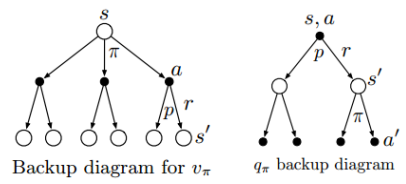
\includegraphics[scale=0.5]{value_functions}
\centering
\caption{Value and State-Value Functions}
\end{figure}

\noindent
Optimal State Value Function. A policy $\pi$ is better
or equal to another policy $\pi^{\prime}$ if its expected return is greater than
or equal to that of $\pi^{\prime}$ for all states ($\pi^{\prime} \geq
\pi^{\prime}$ if and only if $v_{\pi}(s) \geq v_{\pi^{\prime}}(s)$). 

\begin{equation}
v_{*}(s) \doteq \max _{\pi} v_{\pi}(s)
\end{equation}

\noindent
Optimal Action Value Function and its relation to $v_{*}$. Equation 15 gives the
expected return for taking action a in state s and thereafter following an
optimal policy. Comparing with equation 11, $v_{\pi}(s)$ represents the value of
a state as the summation of future returns. In equation 15,
$v_{*}\left(S_{t+1}\right)$ gives the optimal value of all future states from
the given state and action.

\begin{equation}
\begin{aligned}
q_{*}(s, a) &\doteq \max _{\pi} q_{\pi}(s, a)\\
&= \mathbb{E}\left[R_{t+1}+\gamma v_{*}\left(S_{t+1}\right) | S_{t}=s, A_{t}=a\right]
\end{aligned}
\end{equation}

\noindent
Relationship between $q_{*}$ and $v_{*}$. The value of a state under an optimal
policy must equal the expected return for the best action from that state.
Second last line of equation 16 shows that $G_{t} = R_{t+1} + \gamma
v_{*}(S_{t+1})$ when following $\pi_{*}$. The last line is the same as equation
17. For finite MDPs, the last line of equation 16 has a unique solution.

\begin{equation}
\begin{aligned}
v_{*}(s) &=\max _{a \in A(s)} q_{*}(s, a)\\
&= \max _{a} q_{*}(s, a)\\
&= \max _{a} \mathbb{E}_{\pi_{*}}[G_{t} | S_{t} = s, A_{t} = a]\\
&= \max _{a} \mathbb{E}[R_{t+1} + \gamma v_{*}(S_{t+1}) | S_{t} = s, A_{t} = a]\\
&= \max _{a} \sum_{s^{\prime}, r} p(s^{\prime}, r | s, a)[r + \gamma v_{*}(s^{\prime})]
\end{aligned}
\end{equation}


\noindent
Bellman Optimality Equations

\begin{equation}
\begin{aligned}
v_{*}(s) & = \max _{a} \mathbb{E}\left[R_{t+1}+\gamma v_{*}\left(S_{t+1}\right) | S_{t}=s, A_{t}=a\right]\\
&= \max _{a} \sum_{s^{\prime}, r} p\left(s^{\prime}, r | s, a\right)\left[r+\gamma v_{*}\left(s^{\prime}\right)\right]
\end{aligned}
\end{equation}

\begin{equation}
\begin{aligned}
q_{*}(s, a)&=\mathbb{E}\left[R_{t+1}+\gamma \max _{a^{\prime}} q_{*}\left(S_{t+1}, a^{\prime}\right) | S_{t}=s, A_{t}=a\right] \\
&=\sum_{s^{\prime}, r} p\left(s^{\prime}, r | s, a\right)\left[r+\gamma \max _{a^{\prime}} q_{*}\left(s^{\prime}, a^{\prime}\right)\right]
\end{aligned}
\end{equation}

\newpage
\noindent
In $v_{*}$, the next best action is selected based on the expected reward and
value of future states. In $q_{*}$, the state and action is given as well as the
reward. From the new state $s^{\prime}$, the best action is chosen.

\begin{figure}[h]
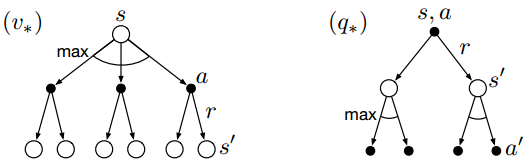
\includegraphics[scale=0.5]{bellman_optimality}
\centering
\caption{Bellman Optimality Equations}
\end{figure}
    
\end{document}
